% \documentclass[handout]{beamer}
\documentclass[aspectratio=169]{beamer}

\mode<presentation>
{
  \usetheme{default}
  % \usefonttheme[onlymath]{serif}
  % \usetheme{Singapore}
  % \usetheme{Warsaw}
  % \usetheme{Malmoe}
  % \useinnertheme{circles}
  % \useoutertheme{infolines}
  % \useinnertheme{rounded}

  \setbeamercovered{transparent=20}
}

\usepackage[english]{babel}
\usepackage[latin1]{inputenc}
\usepackage{alltt,listings,multirow,ulem,siunitx}
\usepackage[absolute,overlay]{textpos}
\TPGrid{1}{1}
\usepackage{pdfpages}
\usepackage{ulem}
\usepackage{multimedia}
\usepackage{multicol}
\usepackage{transparent}
\newcommand\hmmax{0}
\newcommand\bmmax{0}
\usepackage{bm}
\usepackage{comment}
\usepackage{subfig}
% https://tex.stackexchange.com/questions/426088/texlive-pretest-2018-beamer-and-subfig-collide
\makeatletter
\let\@@magyar@captionfix\relax
\makeatother

% font definitions, try \usepackage{ae} instead of the following
% three lines if you don't like this look
\usepackage{mathptmx}
\usepackage[scaled=.90]{helvet}
% \usepackage{courier}
\usepackage[T1]{fontenc}
\usepackage{tikz}
\usetikzlibrary{decorations.pathreplacing}
\usetikzlibrary{shadows,arrows,shapes.misc,shapes.arrows,shapes.multipart,arrows,decorations.pathmorphing,backgrounds,positioning,fit,petri,calc,shadows,chains,matrix}

\newcommand\vvec{\bm v}
\newcommand\bvec{\bm b}
\newcommand\bxk{\bvec_0 \times \kappa_0 \cdot \nabla}
\newcommand\delp{\nabla_\perp}

% \usepackage{pgfpages}
% \pgfpagesuselayout{4 on 1}[a4paper,landscape,border shrink=5mm]

\usepackage{JedMacros}

\newcommand{\timeR}{t_{\mathrm{R}}}
\newcommand{\timeW}{t_{\mathrm{W}}}
\newcommand{\mglevel}{\ensuremath{\ell}}
\newcommand{\mglevelcp}{\ensuremath{\mglevel_{\mathrm{cp}}}}
\newcommand{\mglevelcoarse}{\ensuremath{\mglevel_{\mathrm{coarse}}}}
\newcommand{\mglevelfine}{\ensuremath{\mglevel_{\mathrm{fine}}}}

%solution and residual
\newcommand{\vx}{\ensuremath{x}}
\newcommand{\vc}{\ensuremath{\hat{x}}}
\newcommand{\vr}{\ensuremath{r}}
\newcommand{\vb}{\ensuremath{b}}

%operators
\newcommand{\vA}{\ensuremath{A}}
\newcommand{\vP}{\ensuremath{I_H^h}}
\newcommand{\vS}{\ensuremath{S}}
\newcommand{\vR}{\ensuremath{I_h^H}}
\newcommand{\vI}{\ensuremath{\hat I_h^H}}
\newcommand{\vV}{\ensuremath{\mathbf{V}}}
\newcommand{\vF}{\ensuremath{F}}
\newcommand{\vtau}{\ensuremath{\mathbf{\tau}}}


\title{On Performance Portability for Unstructured High-order Finite Element Computations}
\author{{\bf Jed Brown} and Jeremy Thompson (CU Boulder) \\
  Collaborators: \\
  \quad Jean-Sylvain Camier, Veselin Dobrev, and Tzanio Kolev (LLNL) \\
  \quad Misun Min (ANL) \\
  \quad David Medina (Two Sigma/LLNL) \\
  \quad Kasia Swirydowicz and Tim Warburton (Virginia Tech) \\
  \quad Thilina Rathnayake and Paul Fischer (University of Illinois)}

% - Use the \inst command only if there are several affiliations.
% - Keep it simple, no one is interested in your street address.
% \institute
% {
%   Mathematics and Computer Science Division \\ Argonne National Laboratory
% }

\date{SIAM Annual Meeting, 2018-07-09}

% This is only inserted into the PDF information catalog. Can be left
% out.
\subject{Talks}


% If you have a file called "university-logo-filename.xxx", where xxx
% is a graphic format that can be processed by latex or pdflatex,
% resp., then you can add a logo as follows:

% \pgfdeclareimage[height=0.5cm]{university-logo}{university-logo-filename}
% \logo{\pgfuseimage{university-logo}}



% Delete this, if you do not want the table of contents to pop up at
% the beginning of each subsection:
% \AtBeginSubsection[]
% {
% \begin{frame}<beamer>
%   \frametitle{Outline}
%   \tableofcontents[currentsection,currentsubsection]
% \end{frame}
% }

\AtBeginSection[]
{
  \begin{frame}<beamer>
    \frametitle{Outline}
    \tableofcontents[currentsection]
  \end{frame}
}

% If you wish to uncover everything in a step-wise fashion, uncomment
% the following command:

% \beamerdefaultoverlayspecification{<+->}

\begin{document}
\lstset{language=C}
\normalem

\begin{frame}
  \titlepage
\end{frame}

\setbeamercolor{background canvas}{bg=}

\includepdf[pages=2-3]{figures/ceed/1am/fy17-review.pdf}
\includepdf[pages=7]{figures/ceed/1am/CEED1AM-FuturePlans.pdf} % High Order Software Ecosystem
\includepdf[pages=7]{figures/ceed/1am/fy17-review.pdf} % CEED Software Products
\includepdf[pages=46]{/home/jed/ceed/ceed/talks/CEED-ECP-FY17-Review-Aug-2017.pdf} % Applicable to variety of physics

\begin{frame}[shrink=5]{Performance of assembled versus unassembled}
  \vspace{1ex}
  \includegraphics[width=\textwidth]{figures/TensorVsAssembly} \\
  \begin{itemize}
  \item Arithmetic intensity for $\Qk p$ elements
    \begin{itemize}
    \item $< \frac 1 4$ (assembled), $\approx 10$ (unassembled), $\approx 4$ to $8$ (hardware)
    \end{itemize}
  \item store Jacobian information at Quass quadrature points, can use AD
  \end{itemize}
\end{frame}


\begin{comment}
\begin{frame}{Nekbone}
  \begin{itemize}
  \item Conjugate gradient spectral element benchmark with sum factorization
  \item Without multigrid preconditioner -- a significant and interesting factor for Nek5000
  \end{itemize}
  \includegraphics[width=\textwidth]{figures/ceed/ms8/figures/nekbone/nekbone_rate_vs_time.png}
\end{frame}
\end{comment}

\begin{frame}{Performance versatility: $n_{1/2}$ and $t_{1/2}$}
  \begin{itemize}
  \item Suppose a linear scaling algorithm
  \item Let $r(n)$ be the performance rate (e.g., DOF/second or GF/s) for local problem size $n = N/P$
  \item Let $r_{\max} = \max_n r(n)$ be the peak attainable performance
  \item $ n_{1/2} = \min \{ n : r(n) \ge \frac 1 2 r_{\max} \} $
    \begin{itemize}
    \item Local problem sizes $n < n_{1/2}$ will not yield acceptable efficiency
    \end{itemize}
  \item $ t_{1/2} = 2 n_{1/2} / r_{\max} $
    \begin{itemize}
    \item Time to solution less than $t_{1/2}$ is not feasible with acceptable efficiency
    \end{itemize}
  \end{itemize}
\end{frame}

\begin{frame}{2017 HPGMG performance spectra}
  \begin{center}
    \vspace{-1em}
    \includegraphics[trim=0 5 0 20,clip,width=.8\textwidth]{figures/hpgmg/hpgmg-fv-201706.png}
  \end{center}
\end{frame}

\includepdf[pages=19]{figures/ceed/1am/fy17-review.pdf} % CEED Bake-off problems
\begin{frame}
  \begin{figure} %[!h]
    \centering
    \subfloat[BP1 Nek5000]{{\includegraphics[width=0.35\textwidth]{./figures/ceed/paper1/plot2_Nek5000_bp1_cetus_xlc_N512_pn32.pdf}}}
    \subfloat[BP1 MFEM   ]{{\includegraphics[width=0.35\textwidth]{./figures/ceed/paper1/plot2_MFEM_bp1_v1_cetus_xlc_N512_pn32.pdf}}}
    \subfloat[BP1 deal.II]{{\includegraphics[width=0.35\textwidth]{./figures/ceed/paper1/plot2_deal_II_bp1_cetus_gcc_N512_pn32.pdf}}}
    \caption{\label{bp1_bgq_xlc}BP1 results of Nek5000 (left), MFEM (center), and deal.ii (right)
      on BG/Q with varying polynomial order ($p=1,...,16$) with the number of
      quadrature points ($q=p+2$). The number cpu cores $P=8,192$.}
  \end{figure}
\end{frame}

\begin{frame}{BP1 on KNL: Nek5000 and MFEM}
  \begin{columns}
    \begin{column}{.5\textwidth}
      \includegraphics[width=\textwidth]{figures/ceed/ms6/plot2_Nek5000_bp1_linux_intel_N001_pn32.pdf} \\
      Nek5000 $n_{1/2} = 15k, t_{1/2}= 150\mu s$
    \end{column}
    \begin{column}{.5\textwidth}
      \includegraphics[width=\textwidth]{figures/ceed/ms6/plot2_MFEM_bp1_v1_linux_intel_N001_pn32.pdf} \\
      MFEM $n_{1/2} = 10k, t_{1/2} = 400 \mu s$
    \end{column}
  \end{columns}
  \begin{itemize}
  \item BG/Q has similar performance
  \end{itemize}
\end{frame}

\begin{comment}
\begin{frame}{BP2 on KNL: Nek5000 and MFEM}
  \begin{columns}
    \begin{column}{.5\textwidth}
      \includegraphics[width=\textwidth]{figures/ceed/ms6/plot2_Nek5000_bp2_linux_intel_N001_pn32.pdf} \\
      Nek5000 $n_{1/2} = 30k, t_{1/2} = 300\mu s$
    \end{column}
    \begin{column}{.5\textwidth}
      \includegraphics[width=\textwidth]{figures/ceed/ms6/plot2_MFEM_bp2a_v1_linux_intel_N001_pn32.pdf} \\
      MFEM $n_{1/2} = 15k, t_{1/2} = 300\mu s$
    \end{column}
  \end{columns}
\end{frame}

\begin{frame}{BP1 on Power8: Nek5000 and MFEM}
  \includegraphics[width=.49\textwidth]{figures/ceed/ms6/plot2_Nek5000_bp1_ray_gcc_N001_pn32.pdf}
  \includegraphics[width=.49\textwidth]{figures/ceed/ms6/plot2_MFEM_bp1_v1_ray_gcc_N001_pn32.pdf}
  \begin{itemize}
  \item Nek5000 $t_{1/2} = 75 \mu s$, MFEM $t_{1/2} = 200 \mu s$
  \end{itemize}
\end{frame}

\begin{frame}
  \begin{table}
    \caption{Performance results for various machines using metrics
      defined in Sec. \ref{sec:n12}.
      Each entry corresponds to Nek/MFEM results.
      Results sorted by problem and $t_{\frac{1}{2}}$ performance.}
    \label{tab:bp-summary}
    \begin{center}
      \begin{tabular}{llll}
        Machine/Problem & $r_{max}$ (MDOFs) & $n_{\frac{1}{2}}$ (KDOFs)
        &  $t_{\frac{1}{2}}$ (ms) \\
        \toprule
        Ray/BP1-gcc     & 400/350 & 15/35 & 0.075/0.200 \\
        KNL32/BP1-intel & 200/150 & 15/30 & 0.150/0.400 \\
        KNL32/BP1-gcc   & 100/100 & 20/8  & 0.400/0.160 \\
        Vulcan/BP1-gcc  & \phantom{0}35/40  & 15/10 & 0.857/0.500 \\
        \toprule
        KNL32/BP2-intel & 200/100 & 30/15 & 0.300/0.300 \\
        KNL32/BP2-gcc   & 100/100 & 50/15 & 1.000/0.300 \\
        Vulcan/BP2-gcc  & \phantom{0}35/30  & 21/10 & 1.200/0.666 \\
        \toprule
        Vulcan/BP3-gcc  & \phantom{100}/30 & \phantom{10}/10 & \phantom{0.000}/0.666 \\
        Vulcan/BP3-xlc  & \phantom{100}/20 & \phantom{10}/10 & \phantom{0.000}/1.000 \\
        \toprule
        Vulcan/BP4-gcc  & \phantom{100}/20 & \phantom{10}/10 & \phantom{0.000}/1.000 \\

        \bottomrule
      \end{tabular}
    \end{center}
  \end{table}
\end{frame}
\end{comment}

\includepdf[pages=11]{figures/ceed/1am/fy17-review.pdf} % CEED/OCCA

\begin{frame}{OCCA performance on Summit (V100)}
  \begin{figure}%[!h]
    \centering
    \subfloat[BK1 Summit]{{\includegraphics[width=0.5\textwidth]{./figures/ceed/paper1/bk1_tflops.pdf}}}
    \subfloat[BK3 Summit]{{\includegraphics[width=0.5\textwidth]{./figures/ceed/paper1/bk3_tflops.pdf}}}
    \caption{BK1 and BK3 V100 performance: TFLOPS versus problem size $n$ for
      different polynomial orders, $N$.  Operating on E-vectors (does not include element restriction $\mathcal E, \mathcal E^T$)}
  \end{figure}
\end{frame}

\includepdf[pages=9]{figures/ceed/1am/fy17-review.pdf} % MAGMA batched

\begin{frame}{MPICH CH4: lightweight device layer}
  \begin{itemize}
  \item CH4: faster offload, better fast path/inlining/IPO
  \end{itemize}
  \includegraphics[width=.49\textwidth]{figures/ceed/ms6/figure7_1_nek.pdf}
  \includegraphics[width=.49\textwidth]{figures/ceed/ms6/figure7_2_nek.pdf}
\end{frame}

\begin{frame}{libCEED: Code for Efficient Extensible Discretization}
  \begin{itemize}
  \item BSD-2 license, C library with Fortran interface
  \item Releases: v0.1 (January), v0.2 (March), v0.3 (imminent)
  \item Purely algebraic interface
  \item Extensible backends
    \begin{itemize}
    \item CPU: reference, vectorized
    \item OCCA (just-in-time compilation): CPU, OpenMP, OpenCL, CUDA
    \item MAGMA
    \end{itemize}
  \item Platform for collaboration with vendors
  \item Minimal assumptions about execution environment, parallel decomposition
  \item Primary target: high order finite element methods
    \begin{itemize}
    \item $H^1, H(\mathrm{div}), H(\mathrm{curl})$
    \item also of interest to spectral difference, etc.
    \item Exploit tensor product structure when possible
    \end{itemize}
  \end{itemize}
\end{frame}

\begin{frame}
  \includegraphics[width=\textwidth]{figures/ceed/libCEED-2.pdf}
\end{frame}

\begin{frame}{Quadrature Function}
  \begin{gather*}
    v^T F(u) \sim \int_\Omega v \cdot f_0(u, \nabla u) + \nabla v \tcolon f_1(u, \nabla u) \qquad
    v^T J w \sim \int_\Omega \begin{bmatrix} v \\ \nabla v \end{bmatrix}^T \begin{bmatrix} f_{0,0} & f_{0,1} \\ f_{1,0} & f_{1,1} \end{bmatrix} \begin{bmatrix} w \\ \nabla w \end{bmatrix} \\
    u_e = B \mathcal E_e u \qquad \nabla u_e = \frac{\partial X}{\partial x} B_{\nabla} \mathcal E_e u \\
    J w = \sum_e \mathcal E_e^T \begin{bmatrix} B \\ B_{\nabla} \end{bmatrix}^T
    \underbrace{\begin{bmatrix} I & \\ & \left( \frac{\partial X}{\partial x}\right)^T \end{bmatrix} W_q \begin{bmatrix} f_{0,0} & f_{0,1} \\ f_{1,0} & f_{1,1} \end{bmatrix} \begin{bmatrix} I & \\ & \left( \frac{\partial X}{\partial x}\right) \end{bmatrix}}_{\text{coefficients at quadrature points}} \begin{bmatrix} B \\ B_{\nabla} \end{bmatrix} \mathcal E_e w 
  \end{gather*}
  \begin{itemize}
  \item $B$ and $B_\nabla$ are tensor contractions -- independent of element geometry
  \item Choice of how to order and represent gathers $\mathcal E$ and scatters $\mathcal E^T$
  \item Who computes the metric terms and other coefficients?
  \item Similar for Neumann/Robin and nonlinear boundary conditions
  \end{itemize}
\end{frame}

\begin{frame}[fragile]{Quadrature Functions}
  \begin{itemize}
  \item Multiple inputs and outputs
  \item Independent operations at each of \texttt{Q} quadrature points
  \item Ordering and number of elements not specified
  \end{itemize}
  \begin{minipage}{0.5\textwidth}
    \begin{minted}{C}
      int L2residual(void *ctx, CeedInt Q,
                     const CeedScalar *const in[],
                     CeedScalar *const out[]) {
        const CeedScalar *u = in[0], *rho = in[1], *target = in[2];
        CeedScalar *v = out[0];
        for (CeedInt i=0; i<Q; i++)
          v[i] = rho[i] * (u[i] - target[i]);
        return 0;
      }
    \end{minted}
  \end{minipage}
\end{frame}

\begin{comment}
\begin{frame}{High-level API Proposal}
  \begin{gather*} v^T J w = \sum_e \mathcal E_e^T \begin{bmatrix} B \\ D \end{bmatrix}^T
    \underbrace{\begin{bmatrix} I & \\ & \left( \frac{\partial X}{\partial x}\right)^T \end{bmatrix} W_q \begin{bmatrix} f_{0,0} & f_{0,1} \\ f_{1,0} & f_{1,1} \end{bmatrix} \begin{bmatrix} I & \\ & \left( \frac{\partial X}{\partial x}\right) \end{bmatrix}}_{\text{coefficients at quadrature points}} \begin{bmatrix} B \\ D \end{bmatrix} \mathcal E_e w
  \end{gather*}
  \begin{itemize}
  \item Proposal:
    \begin{itemize}
    \item Setup: specify $\mathcal E$ and local ordering choice for $f$
    \item Apply: implementation handles batching, work buffers, and calling $f(u, \nabla u)$.
    \end{itemize}
  \item User links to interface library
  \item Backend implementation switchable at run-time
  \item Two-phase implementation enables connectivity analysis and JIT
  \end{itemize}
\end{frame}
\end{comment}

\begin{frame}{Element restriction $\mathcal E_e$}
  \begin{itemize}
  \item Conforming homogeneous mesh: boolean matrix with homogeneous block size
  \item Non-conforming mesh: anchored rows have linear combination
  \item Nek5000-style E-vector: indexed identity
  \item libCEED backends are allowed to reorder, compress, etc.
  \item May be applied all at once or in batches
  \end{itemize}
\end{frame}

\begin{frame}[fragile]{libCEED Operator}
  \begin{equation*}
    A = \mathcal P^T \underbrace{\mathcal E^T B D B \mathcal E}_{\text{CeedOperator}} \mathcal P
  \end{equation*}
  \begin{itemize}
  \item element restriction $\mathcal E$, basis $B$, quadrature function $D$
  \end{itemize}
  \begin{minipage}{0.5\textwidth}
    \begin{minted}{C}
      CeedOperatorCreate(ceed, qf_L2residual, &op);
      CeedOperatorSetField(op, "u", E, Basis, CEED_VECTOR_ACTIVE);
      CeedOperatorSetField(op, "rho", CEED_RESTRICTION_IDENTITY,
                           CEED_BASIS_COLOCATED, rho);
      CeedOperatorSetField(op, "target", CEED_RESTRICTION_IDENTITY,
                           CEED_BASIS_COLOCATED, target);
      CeedOperatorSetField(op, "v", E, Basis, CEED_VECTOR_ACTIVE);
    \end{minted}
  \end{minipage}
\end{frame}

\begin{frame}{Vectorization techniques}
  \begin{itemize}
  \item Vectorize within a single high-order element
    \begin{itemize}
    \item Minimal working set (as small as one element)
    \item Specialized implementation for different degree/\# quadrature points
    \item Hard to avoid cross-lane operations at modest degree
    \item Nek5000
    \end{itemize}
  \item Vectorize across elements in batches \texttt{[i,j,k,e]}
    \begin{itemize}
    \item Working set has at least vector length number of elements (e.g., 8)
    \item Generic implementation is easy to optimize; no cross-lane operations
    \item HPGMG-FE, Deal.II (Kronbichler and Kormann), MFEM (new)
    \end{itemize}
  \end{itemize}
\end{frame}

\begin{frame}{MFEM vectorization performance}
  \begin{figure}%[!h]
    \centering
    \subfloat[Cetus internal vectorization]{{\includegraphics[width=0.5\textwidth]{./figures/ceed/plot2_MFEM_bp1_v1_cetus_xlc_N512_pn32.pdf}}}
    \subfloat[Cetus external vectorization]{{\includegraphics[width=0.5\textwidth]{./figures/ceed/plot2_MFEM_bp1_v1_cetus_xlc_N512_pn32_evec.pdf}}}
    \caption{Internal versus external element vectorization for BP1.}
  \end{figure}
\end{frame}

\begin{frame}{HPGMG: a benchmark for supercomputers}
  \begin{itemize}
  \item \url{https://hpgmg.org}
  \item Mark Adams, Sam Williams (finite-volume), Jed (finite-element), John Shalf, Brian Van Straalen, Erich Strohmeier, Rich Vuduc
  \item Annual BoFs at Supercomputing since 2014
  \item Implementations
    \begin{description}
    \item[Finite Volume] memory bandwidth intensive, simple data dependencies, 4th order
    \item[Finite Element] compute- and cache-intensive, vectorizes, overlapping writes
    \end{description}
  \item Full multigrid, well-defined, scale-free problem
  \item Matrix-free operators, Chebyshev smoothers
  \end{itemize}
\end{frame}

\begin{frame}[fragile]
  \frametitle{Full Multigrid (FMG): Prototypical Fast Algorithm}
  \begin{figure}
  \centering
  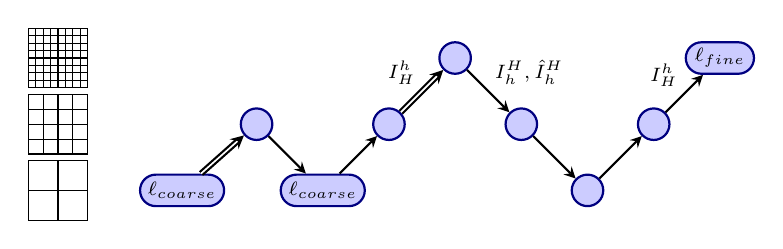
\begin{tikzpicture}
    [>=stealth,
    every node/.style={inner sep=2pt},
    restrict/.style={thick},
    prolong/.style={thick},
    mglevel/.style={rounded rectangle,draw=blue!50!black,fill=blue!20,thick,minimum size=4mm},
    ]
    \begin{scope}\scriptsize
      \newcommand\mgdx{3.0em}
      \newcommand\mgdy{3.0em}
      \newcommand\mgl[1]{(pow(2,#1+1))}
      \newcommand\mgloc[4]{(#1 + #4*\mgdx*#3,#2 + \mgdy*#3)}

      \node[mglevel] (coarseinit) at \mgloc{-3}{0}{0}{0} {$\mglevel_{coarse}$};

      \node[mglevel] (afine) at \mgloc{0}{0}{1}{1} {};

      \node[mglevel] (bcoarse) at \mgloc{2*\mgdx}{0}{0}{1} {$\mglevel_{coarse}$};
      \node[mglevel] (bup1) at \mgloc{2*\mgdx}{0}{1}{1} {};
      \node[mglevel] (bfine) at \mgloc{2*\mgdx}{0}{2}{1} {};

      \node[mglevel] (cdown1) at \mgloc{6*\mgdx}{0}{1}{-1} {};
      \node[mglevel] (ccoarse) at \mgloc{6*\mgdx}{0}{0}{-1} {};
      \node[mglevel] (cup1) at \mgloc{6*\mgdx}{0}{1}{1} {};
      \node[mglevel] (cfine) at \mgloc{6*\mgdx}{0}{2}{1} {$\mglevel_{fine}$};


      \draw[->,restrict,double]
                         (coarseinit) -- node [above right] {} (afine);
      \draw[->,restrict]
                         (afine) -- node [above right] {} (bcoarse);
      \draw[->,restrict]
                         (bcoarse) -- node [above right] {} (bup1);
      \draw[->,restrict,double]
                         (bup1) -- node [above left] {$\mathbb I_H^h$} (bfine);
      \draw[->,restrict]
                         (bfine) -- node [above right] {$I_h^H,\hat I_h^H$} (cdown1);
      \draw[->,restrict]
                         (cdown1) -- node [above right] {} (ccoarse);
      \draw[->,restrict]
                         (ccoarse) -- node [above right] {} (cup1);
      \draw[->,restrict]
                         (cup1) -- node [above left] {$I_H^h$} (cfine);

      %grids
      \newcommand\mghx{0.9*\mgdx}
      \newcommand\mghy{0.9*\mgdy}

      \draw[shift=\mgloc{-2*\mgdx}{0}{2}{0},
      xstep=\mghy/\mgl{2},
      ystep=\mghy/\mgl{2}]
      (-0.5*\mghy,-0.5*\mghy) grid (0.5*\mghy,0.5*\mghy);

      \draw[shift=\mgloc{-2*\mgdx}{0}{1}{0},
      xstep=\mghy/\mgl{1},
      ystep=\mghy/\mgl{1}]
      (-0.5*\mghy,-0.5*\mghy) grid (0.5*\mghy,0.5*\mghy);

      \draw[shift=\mgloc{-2*\mgdx}{0}{0}{0},
      xstep=\mghy/\mgl{0},
      ystep=\mghy/\mgl{0}]
      (-0.5*\mghy,-0.5*\mghy) grid (0.5*\mghy,0.5*\mghy);

  \end{scope}
\end{tikzpicture}
\label{fig:FMG}
\end{figure}
\begin{itemize}
  \item start with coarse grid
  \item truncation error within one cycle
  \item about five work units for many problems
  \item no ``fat'' left to trim -- robust to gaming
  \item distributed memory -- restrict active process set using Z-order
    \begin{itemize}
    \item $\bigO(\log^2 N)$ parallel complexity stresses network
    \end{itemize}
  \item scale-free specification
    \begin{itemize}
    \item no mathematical reward for decomposition granularity
    \item don't have to adjudicate ``subdomain''
    \end{itemize}
\end{itemize}
\end{frame}

\begin{comment}
  \begin{frame}{Multigrid design decisions}
  \begin{itemize}
  \item $Q_2$ finite elements
    \begin{itemize}
    \item Partition of work not partition of data -- sharing/overlapping writes
    \item $Q_2$ is a middle-ground between lowest order and high order
    \item Matrix-free pays off, tensor-product element evaluation
    \end{itemize}
  \item Linear elliptic equation with manufactured solution
  \item Mapped coordinates
    \begin{itemize}
    \item More memory streams, increase working set, longer critical path
    \end{itemize}
  \item No reductions
    \begin{itemize}
    \item Coarse grid is strictly more difficult than reduction
    \item Not needed because FMG is a direct method
    \end{itemize}
  \item Chebyshev/Jacobi smoothers, $V(3,1)$ cycle
    \begin{itemize}
    \item Multiplicative smoothers hard to verify in parallel
    \item Avoid intermediate scales (like Block Jacobi/Gauss-Seidel)
    \end{itemize}
  \item Full Approximation Scheme
  \end{itemize}
\end{frame}
\end{comment}

\begin{frame}{HPGMG-FE on Edison, SuperMUC, Titan}
  \begin{center}
    \vspace{-1em}
    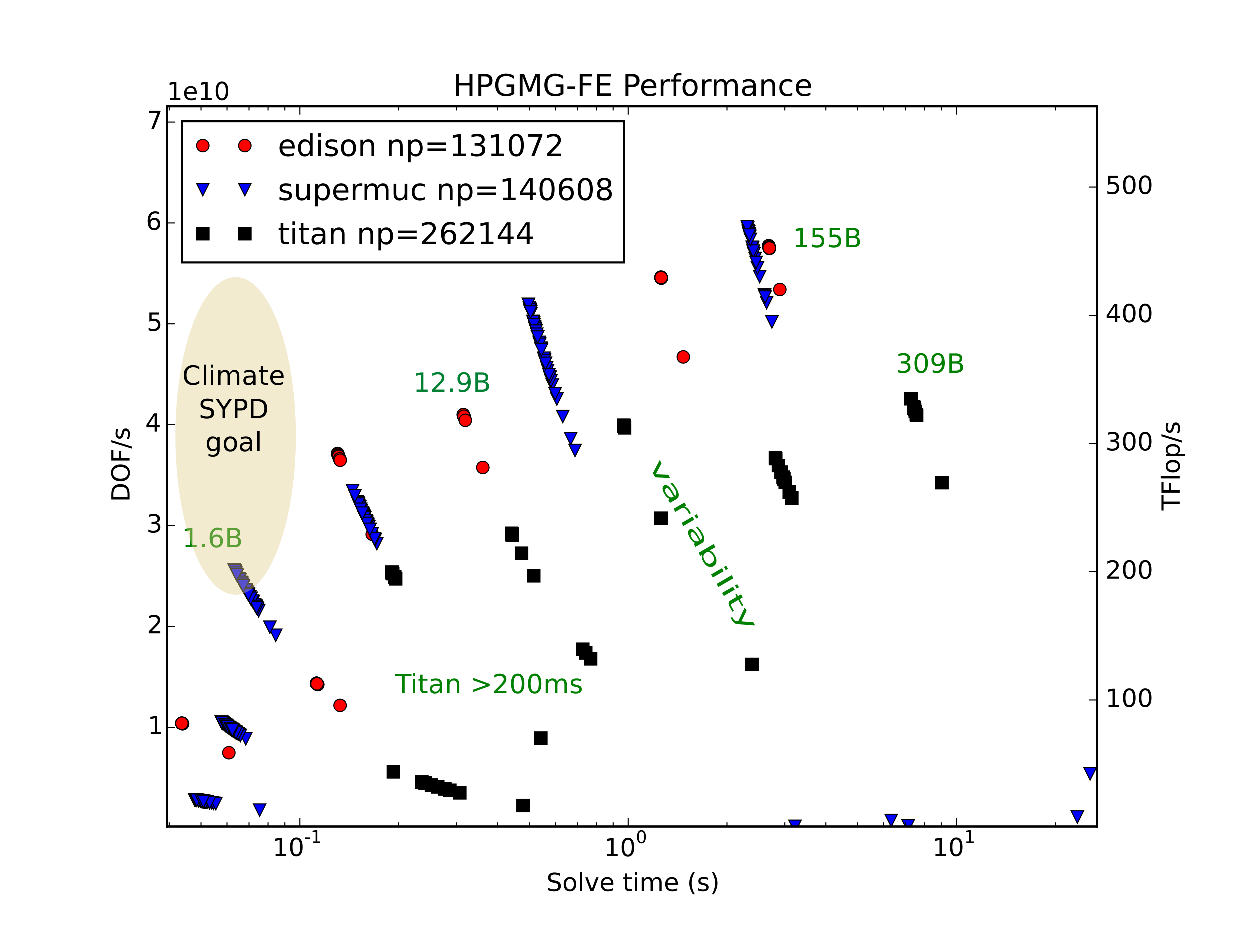
\includegraphics[trim=0 10 0 20,clip,width=.8\textwidth]{figures/hpgmg/range-edison-supermuc-titan-ann2.eps}
  \end{center}
\end{frame}

\begin{frame}{Outlook}
  \begin{itemize}
  \item libCEED is interested in contributors and friendly users
  \item GPU performance optimizations in progress
  \item Cache versus vectorization tradeoffs
    \begin{itemize}
    \item Backends should automatically choose internal versus external vectorization
    \item Choice depends on architecture, element size, number of fields
    \end{itemize}
  \item Throughput versus latency optimizations
  \item Even/odd performance optimization
  \item Incorporate algorithmic differentiation
  \item Developing exchange/storage interfaces for high-order fields
  \item Many other activities to improve high order ecosystem
  \end{itemize}
\end{frame}

\end{document}
